\documentclass[11pt,a4paper]{article}
\usepackage[hyperref]{acl2018}
\usepackage{amsmath}
\usepackage{graphicx}
\usepackage{amsfonts}
\usepackage{times}
\usepackage{latexsym}
\usepackage{placeins}
\usepackage{subfig}

\usepackage{url}

\aclfinalcopy

\title{Using Geospatial Data to Find Investment Opportunities in the Real Estate Market}

\author{Chih Huang \\
  {\tt huangcs} \\
  {\tt @seas.upenn.edu} \\\And
  Ignacio Navarro \\
  {\tt inavarro} \\
  {\tt @seas.upenn.edu} \\\And
  Nikhil Ramesh \\
  {\tt nramesh} \\
  {\tt @seas.upenn.edu}
}

\date{\today}

\begin{document}
\maketitle
\begin{abstract}
  Valuating real estate properties is driven by a series of direct 
  factors (total square area, number of bedrooms, garage spaces, etc) 
  and indirect factors (crime rate, quality of school district, etc). However, private sellers tend to focus more on the former when setting 
  a listing price for their property. In particular, there are many
  geospatial features indirectly related to the property that sellers
  might easily overlook. Proximity to a church, a river, or a police
  station are all factors that play a role, albeit minor, in the valuation
  of a property. In this paper we determine by running a series of models on a dataset consiting
  on properties in South Philadelphia if geographical features do indeed play a decisive role 
  in the valuation of a property. 
\end{abstract}

\section{Introduction}

\subsection{Motivation}

Traditionally, real estate valuation has concentrated on assessing the
features directly surrounding the property to come up with a price.
Straightforward features such as number of bedrooms, whether the property
has a pool or a garage space, or even the number of bathrooms play a major
contribution on the price. And while that does play an important role, private
sellers may not fully realize that the property's surroundings can also
play a role. Points of interest like supermarkets, museums, parks, cafes,
or police stations can affect house prices but many times these may be
overlooked. 

\subsection{Problem Definition}

With all of this in mind the natural question becomes: given all the 
geospatial data related to a property, can a machine learning model 
predict the real value of a property as a \textbf{regression} problem? 
And if so, can one use this to
find investment opportunities in the real estate market? Throughout
this paper we will answer the former question. The latter is a simple
corollary of the former. Indeed, if there is a model that can accurately 
predict house prices given geospatial and direct features, one can use these
results to find investments opportunities by comparing the listing
price on properties currently on the market with what the best model 
predicts the value is and seeing if the property is really undervalued.

\medskip

In other words, let $M: X \to \mathbb{R}^+$ be an accurate model (we will
define what constitutes ``accurate'' to our use case in the next section),
where $X$ is the feature space that constitutes direct and indirect
features related to a property. Given a property $p$ with a listing price of $s_p$ and a set of features $x_p$, we will buy the property if

\begin{equation}
  M(x_p) > s_p
\end{equation}

because $p$ is undervalued.

\subsection{Related Work}

A lot of work has been done in the last few years on predicting house prices
using machine learning. Traditional models have relied in hedonic
regression, a type of regression which breaks the property apart into its direct factors in order to establish
a relationship between the factors and the price of the property. A paper using this method have been 
presented by \cite{jiang2014new} focusing on properties in Singapore with property sales between 1995 and 2014.

\medskip

Our main source for our project is \cite{bergadano2019learning},
in which they analyze a dataset consiting of properties in Madrid, Spain.
There are similarities to what we're trying to investigate: the paper models
the question as a regression problem and uses similar models to the ones we train. 
The main difference, however, is that they only consider direct features for their models. 
The main novelty in our project is to combine these features with geospatial features.
As far as we have researched, no work has investigated our proposal.


\section{Data Acquisition and Exploration}

\subsection{Acquisition}

The acquisition of the dataset for this project consisted on finding basic property
information for Philadelphia that included direct features, and merging this dataset
with all the geospatial information related to the property. The first part was
relatively easy, as \url{https://www.opendataphilly.org/} provided basic information
for over 250,000 properties in Philadelphia. The main challenge was in fact finding
the geographical features. Our approach to solve this was to find APIs that offered
nearest distance to points of interests. Once we found some reliable APIs for this task
(e.g. GoogleMaps API, TomTom API, or FourSquare API), we began the process of merging
the data to our property dataset.

\medskip

The main obstacle of this part, and probably of the project,
was the API rate limit each service offered. Conservatively
speaking, we needed to make
$$
\underbrace{250,000}_{\text{properties}} \times
\underbrace{24}_{\text{geo features}} = 6,000,000 \; \text{API calls}
$$
and unfortunately most of the services offered 1,000 API
calls limit per day. The solution to this part was to
drastically reduce the size of the dataset to around
8,000 properties in South Philadelphia, and even this
amount posed some architectural challenges: we distributed
the API calls for each member of the group and remerged them later. We encourage the reader to look at the code dealing
with this on the project's \href{https://github.com/nachonavarro/real-estate-ml}{repo}, in particular 
the \texttt{properties/data} package.

\subsection{Features}

The list of final features that we feed our model are in
Table \ref{tab:features} for a total of 5 categorical
and 28 numerical (nearest point of interest in meters).

\begin{table}[]
\centering
\begin{tabular}{|l|l|}
\hline
\textbf{Feature} & \textbf{Type} \\ \hline
Fireplaces       & categorical   \\ 
Garage Spaces             & categorical \\ 
Bathrooms                 & categorical \\ 
Bedrooms                  & categorical \\ 
Stories                   & categorical \\ 
Total Area                & numerical   \\ 
Total Livable Area        & numerical   \\ 
Latitude                  & numerical   \\ 
Longitude                 & numerical   \\ 
Nearest Museum            & numerical   \\ 
Nearest Gas Station       & numerical   \\ 
Nearest Coffee Shop       & numerical   \\ 
Nearest Stadium           & numerical   \\ 
Nearest Food              & numerical   \\ 
Nearest Bar               & numerical   \\ 
Nearest Gym               & numerical   \\ 
Nearest Bridge            & numerical   \\ 
Nearest Garden            & numerical   \\ 
Nearest Park              & numerical   \\ 
Nearest River             & numerical   \\ 
Nearest City Hall         & numerical   \\ 
Nearest Police Station    & numerical   \\ 
Nearest Hospital          & numerical   \\ 
Nearest Elementary School & numerical   \\ 
Nearest Church            & numerical   \\ 
Nearest Bank              & numerical   \\ 
Nearest Supermarket       & numerical   \\ 
Nearest Pharmacy          & numerical   \\ 
Nearest Bus Stop          & numerical   \\ 
Nearest Metro Station     & numerical   \\ 
Nearest Train Station     & numerical   \\ 
Nearest University        & numerical   \\ 
Nearest Laundromat        & numerical   \\ \hline
\end{tabular}
\caption{Features used}
\label{tab:features}
\end{table}

\subsection{Exploration}

Once we acquired the data the next step was to explore it
to fully understand it. Some significant results to show are
the following.

\medskip

The distribution of the properties by sale price in South Philadelphia can be seen in Figure \ref{fig:distribution}.
Clearly the distribution is skewed with a mean sale
price of \$324,662.

\begin{figure}[h]
\centering
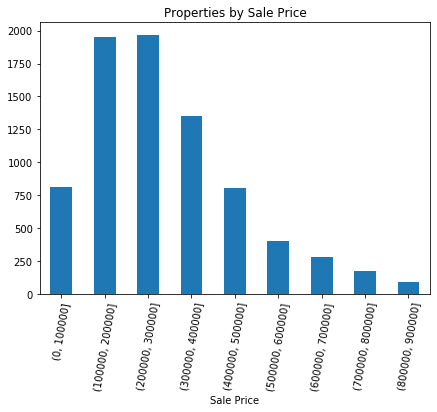
\includegraphics[width=0.5\textwidth]{result-data/properties_sale_price}
\caption{Distribution by sale price}
\label{fig:distribution}
\end{figure}

We can also get a sense of where the properties are located
by plotting a heatmap of South Philadelphia based on
sale price (Figure \ref{fig:heatmap}).

\begin{figure}[h]
\centering
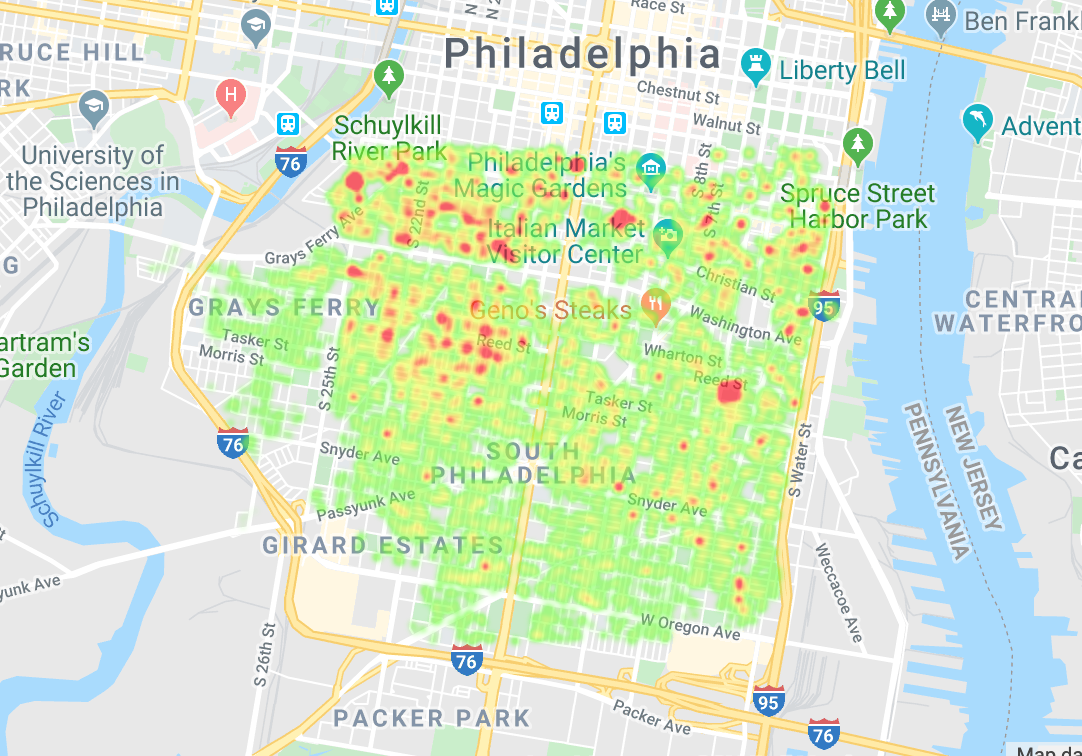
\includegraphics[width=0.5\textwidth]{result-data/heatmap}
\caption{Heatmap of South Philadelphia (hotter means higher
sale price)}
\label{fig:heatmap}
\end{figure}

Another important step was to see the relationship
between the features. To do this we used a correlation
matrix which can be seen in Figure \ref{fig:corr}. For instance, there is a strong correlation between the number of bathrooms and the total livable area. There's also some interesting relationships, e.g., there is negative correlation between the total livable area and the nearest laundromat, which makes (some) sense, as bigger houses in richer neighborhoods don't need laundromats.


\begin{figure}[h]
\centering
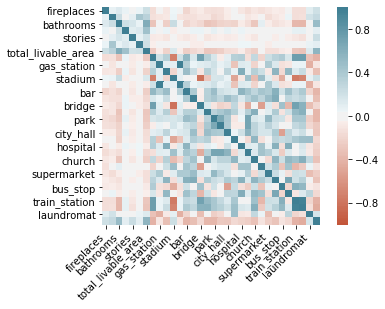
\includegraphics[width=0.5\textwidth]{result-data/correlation_matrix}
\caption{Correlation matrix}
\label{fig:corr}
\end{figure}


\section{Models}

\subsection{Experimental Models Setup}

We wanted to formulate this as a regression problem by using \textbf{sale price} as a target label and training on the features collected for our housing dataset. To do this, we decided to train the following 5 different regression models: Support Vector Regression, Linear Regression, Multi-Layer Perceptron, Regression Tree and KNeighbor Regression.

\medskip

From here, we wanted to evaluate our model in a meaningful way without looking at an MSE Error value that is visually insignificant to us. Additionally, we needed a relative error metric since a \$50,000 error on a \$100,000 property is much worse than a \$50000 error on a \$1,000,000 property. We used our own error metric which classifies a prediction as good if a predicted sale price is within a given tolerance (e.g. 20\%) of the ground-truth sale price and bad otherwise. 

\medskip

We initially trained one model on the entire training dataset but saw that this treated the higher priced houses as outliers. To account for this, we segmented the training data into three segments (cheap, moderate, expensive) and fit a separate model for each segment, resulting in 3 models to cover the entire dataset. This works because our project aims to predict how much a house on the market is actually worth; we should featurize a currently listed house and then based on its list price set by the owner, we place it into the ``cheap'', ``moderate'' or ``expensive'' bucket; then, the corresponding model predicts its worth so we can see if it is being undervalued or overvalued. The key assumption we make here is that the predicted \textit{Sale Price} should not deviate from the bucket that the \textit{List Price} was placed into. 
We see now our experimental findings below.

\subsection{Results and Findings}

\begin{figure}[h]
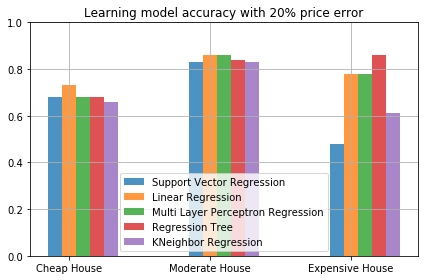
\includegraphics[width=0.5\textwidth]{result-data/tolerance20.png}
\caption{Accuracy comparison for five learning models which are used to predict the cheap, moderate, expensive properties.}
\label{fig:tolerance20}
\centering
\end{figure}
Using the geospatial features and direct factors (number of bedrooms, spaces, etc) to train five learning models with a 20\% tolerance for each model is listed in Figure~\ref{fig:tolerance20}. According to the result, the five models have almost the same accuracy to predict cheap properties and moderate properties. However, there we consistently see three models (Linear Regression, Multi-Layer Perceptron Regression and Regression Tree) that have better accuracy to predict expensive house. 

\subsection{Finding the Best Model}
We took these three models and retrained using a lower tolerance (15\%). The result is shown in Figure~\ref{fig:tolerance15}. 
\begin{figure}[h]
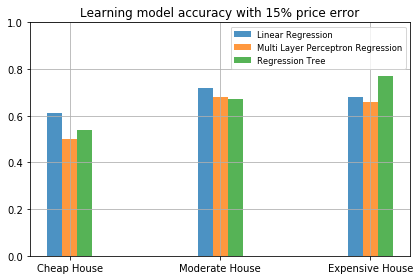
\includegraphics[width=0.5\textwidth]{result-data/tolerance15.png}
\caption{Accuracy comparison for three learning models which have better performance in previous prediction result.}
\label{fig:tolerance15}
\centering
\end{figure}

\begin{figure}[h]
    \centering
    \subfloat[Prediction data for cheap house]{%
        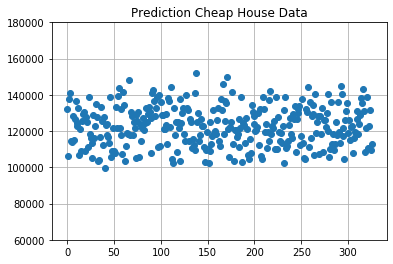
\includegraphics[width=0.24\textwidth]{result-data/linear25p.png}%
        \label{fig:a}%
    }%
    \hfill%
    \subfloat[Test data for cheap house]{%
        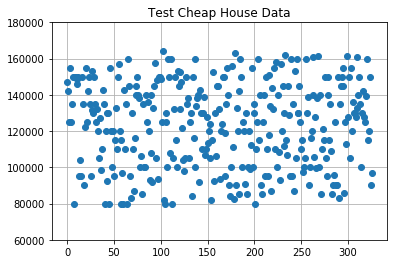
\includegraphics[width=0.24\textwidth]{result-data/linear25t.png}%
        \label{fig:b}%
    }
    \caption{Prediction and test data distribution comparison for cheap house by using linear regression model.}
    \label{fig:linearcheap}
\end{figure}

The accuracy decreased with a tolerance of 15\% for three models, and by inspection we see that Linear Regression and Regression Tree model have a better accuracy than Multi-Layer Perceptron Regression. Furthermore, we analyzed the prediction data and test data distribution to visually see the resemblence between the training and the test data distribution
given a model. For instance, the prediction data distribution are shown in Figure~\ref{fig:linearcheap}, Figure~\ref{fig:linearmoderate}, Figure~\ref{fig:linearexpensive} for different models.

\begin{figure}[h]
    \centering
    \subfloat[Prediction data for moderate house]{%
        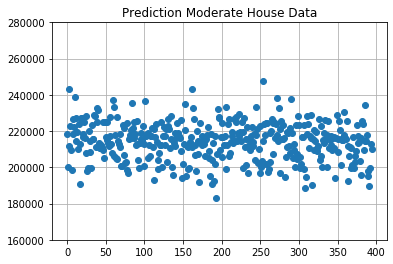
\includegraphics[width=0.24\textwidth]{result-data/linear50p.png}%
        \label{fig:a}%
    }%
    \hfill%
    \subfloat[Test data for moderate house]{%
        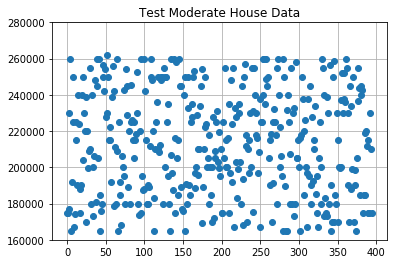
\includegraphics[width=0.24\textwidth]{result-data/linear50t.png}%
        \label{fig:b}%
    }
    \caption{Prediction and test data distribution comparison for moderate house by using linear regression model.}
    \label{fig:linearmoderate}
\end{figure}

According the result which are shown in the figure, Linear Regression model predict the cheap and moderate properties price in a small range which can't represent the true test data. Only expensive house result have the similar distribution between prediction and test data.

\begin{figure}[h]
    \centering
    \subfloat[Prediction data for expensive house]{%
        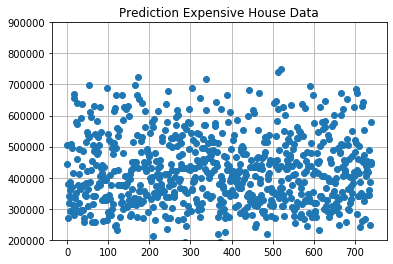
\includegraphics[width=0.24\textwidth]{result-data/linear75p.png}%
        \label{fig:a}%
    }%
    \hfill%
    \subfloat[Test data for expensive house]{%
        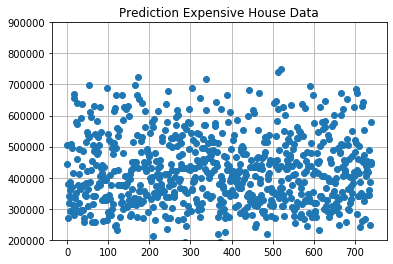
\includegraphics[width=0.24\textwidth]{result-data/linear75p.png}%
        \label{fig:b}%
    }
    \caption{Prediction and test data distribution comparison for expensive house by using linear regression model.}
    \label{fig:linearexpensive}
\end{figure}


\FloatBarrier
After comparing the distribution for the training data and the test data by using Linear Regression model, we then examined the data distribution result by using regression tree learning model. The data distribution is listed in Figure~\ref{fig:regtreecheap}, Figure~\ref{fig:regtreemoderate}, Figure~\ref{fig:regtreemexpensive}. We can see the data is pretty consistent for the three ranges of properties. 

\begin{figure}[h]
    \centering
    \subfloat[Prediction data for cheap house]{%
        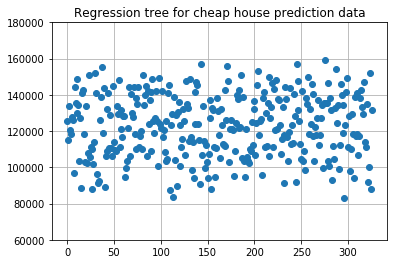
\includegraphics[width=0.24\textwidth]{result-data/regtree25p.png}%
        \label{fig:a}%
    }%
    \hfill%
    \subfloat[Test data for cheap house]{%
        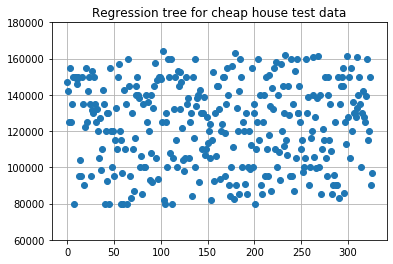
\includegraphics[width=0.24\textwidth]{result-data/regtree25t.png}%
        \label{fig:b}%
    }
    \caption{Prediction and test data distribution comparison for cheap house by using regression tree model.}
    \label{fig:regtreecheap}
\end{figure}
\begin{figure}[h]
    \centering
    \subfloat[Prediction data for moderate house]{%
        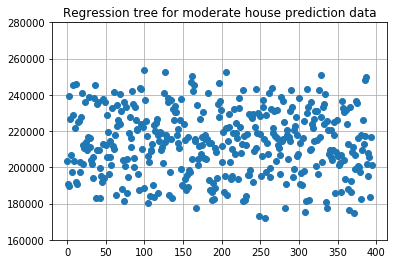
\includegraphics[width=0.24\textwidth]{result-data/regtree50p.png}%
        \label{fig:a}%
    }%
    \hfill%
    \subfloat[Test data for moderate house]{%
        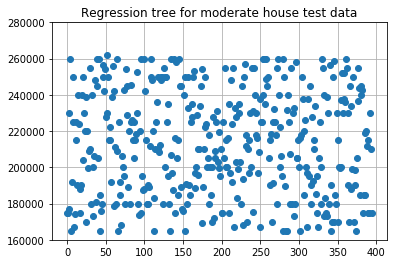
\includegraphics[width=0.24\textwidth]{result-data/regtree50t.png}%
        \label{fig:b}%
    }
    \caption{Prediction and test data distribution comparison for moderate house by using regression tree model.}
    \label{fig:regtreemoderate}
\end{figure}
\FloatBarrier
By examining the two best model and analyze the data distribution for prediction and test data, regression tree model can capture the properties price distribution characteristics. Therefore, the best model to predict the house price will be regression tree model by using our features to train.
\FloatBarrier
\begin{figure}[h]
    \centering
    \subfloat[Prediction data for expensive house]{%
        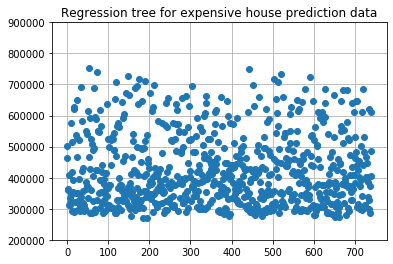
\includegraphics[width=0.24\textwidth]{result-data/regtree75p.png}%
        \label{fig:a}%
    }%
    \hfill%
    \subfloat[Test data for expensive house]{%
        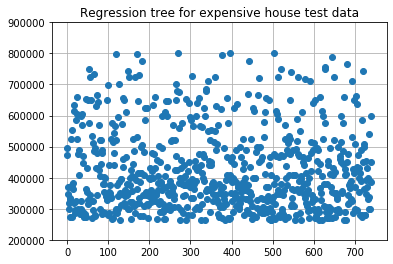
\includegraphics[width=0.24\textwidth]{result-data/regtree75t.png}%
        \label{fig:b}%
    }
    \caption{Prediction and test data distribution comparison for expensive house by using regression tree model.}
    \label{fig:regtreemexpensive}
\end{figure}



\FloatBarrier



\section{Conclusion}

From our models we were able to see that Regression Tree was able to perform the best from training on our features. Under the hood, we checked to see which features it prioritized and were able to find that the geospatial attributes that the most important were 'bus\_stop', 'laundromat', 'university', 'park', 'river', 'train\_station' and 'stadium'. These were in some cases even more important than the direct features. This shows that the collected geospatial features do have an impact in determining housing prices as our best models weighted them heavily.

\medskip

Our most important finding here was the model's improvement in accuracy while using geospatial features over using only the direct features (such as livable area, bedrooms, etc.). We found that the test accuracy increased on average by around 30\% just by adding these new features. This gives us the result we were looking for: geospatial features do have a significant impact on property sale price. 

\medskip

Despite this finding, our models trained on the geospatial features did not perform well enough to accurately predict the true value of housing prices as the accuracy only reached about 70\% on relatively high tolerance thresholds of 15-20\%. This could be because of hidden variables that overpower our collected features, such as crime rate, quality of school district, etc. that we don’t consider. As such, we conclude that geospatial features do have an impact on property sale prices but are not sufficient on their own to predict house prices, although it’s a great initial feature space to investigate and adding additional types of features would only improve a resulting model’s usability in real-world scenarios.

\subsection{Future Work}

Some work that can be done on this project includes adding these hidden factors such as crime rate and school district quality that may increase the effectiveness of our model as well as the usefulness of the geospatial features we've provided.

\medskip

Additionally, we can try some more powerful regression models that may be able to capture the solution to our problem better; for this project, we used the same models as the ones in the paper for Madrid housing \cite{bergadano2019learning} but we may be able to do better.

\medskip

Lastly, we can also compare our trained model with an existing industry model such as Zillow's and see how close we are to emulating their price prediction.

\bibliographystyle{acl_natbib}
\bibliography{acl2018}

\end{document}
